\documentclass[11pt]{article}

\usepackage[margin=2cm]{geometry}
\usepackage{titling}
\usepackage[T1]{fontenc}
\usepackage{tabularx}
\usepackage{amsfonts}
\usepackage{amsmath}
\usepackage{graphicx}
\usepackage{changepage}
\usepackage{algorithm}
\usepackage[noend]{algpseudocode}


\pretitle{\begin{center}\Huge\bfseries}
\posttitle{\par\end{center}\vskip 0.5em}
\preauthor{\begin{center}\Large}
\postauthor{\end{center}}
\predate{\par\large\centering}
\postdate{\par}

\title{Obliczenia naukowe - lab 3}
\author{Jakub Musiał 268442}
\date{Listopad 2023}

\begin{document}

\maketitle

\hspace{1cm}

\section*{Zadania 1-3: Implementacja metod obliczających przybliżenia pierwiastków}
    \subsection*{Problem}
        Zaimplementować funkcje obliczające przybliżenie pierwiastka funkcji $f$ 
        z dokkładnością obliczeń określoną przez $\delta$ oraz $\varepsilon$.
        \newline
        Funkcje mają zwracać czwórkę $(r, v, it, err)$, gdzie: $r$ - przybliżenie pierwiastka $f$, 
        $v$ - wartość $f(r)$, $it$ - liczba iteracji algorytmu, $err$ - sygnalizacja błędu.

        \subsubsection*{Zadanie 1: Metoda biseckcji}
            Metoda znajduje pierwiastek funkcji $f$ w przedziale $[a, b]$, jeśli jest w tym przedziale ciągła
            oraz zmienia znak (brak zmiany znaku skutkuje zwróceniem błędu). Metoda w każdej iteracji wyznacza 
            nowe przybliżenie pierwiastka $f$, obliczając środek $c = \frac{a + b}{2}$ akutalnego przedziału. 
            Jeśli $f(c) \approx 0 \lor |a - b| < \delta$ metoda kończy działanie. W przeciwnym przypadku
            aktualizowany jest przedział $[a, b]$ - jeśli funkcja zmienia znak w przedziale $[a, c]$, to $b \gets c$,
            jeśli natomiast funkcja zmienia znak w przedziale $[c, b]$, to $a \gets c$. 
            \newline
            \begin{figure}[h]
                \centering
                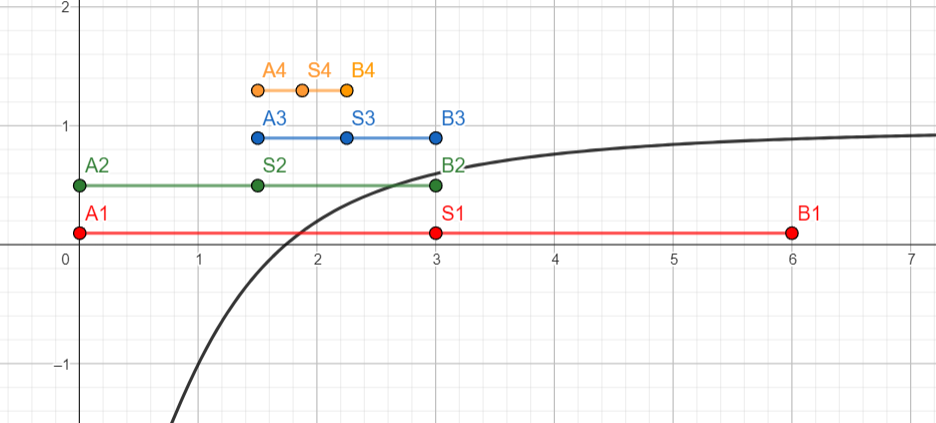
\includegraphics[scale=0.6]{img/bisection.png}
                \caption{Wizualizacja metody bisekcji}
                \label{fig:bisection}
            \end{figure}

        \subsubsection*{Zadanie 2: Metoda stycznych (Newtona)}
            Metoda wyznacza kolejne przybliżenia pierwiastka funkcji $f$ jako argumenty punktów przecięcia z osią $x$ 
            stycznych do funkcji $f$ w punktach $(x_n, f(x_n))$ , zaczynając od zadanego $x_0$ oraz znając pochodną $f'$. 
            Te punkty przecięcia wyznaczane są wg. wzoru $x_{n + 1} = x_n - \frac{f(x_n)}{f'(x_n)}$. Warunkiem 
            końca metody stycznych jest osiągnięcie wymaganej precyji ($|x_{n + 1} - x| < \delta \lor |f(x_{n + 1})| < \varepsilon$) 
            lub wykonanie maksymalnej liczby iteracji $M$ zadanej jako parametr funkcji.
            \newline
            \begin{figure}[h]
                \centering
                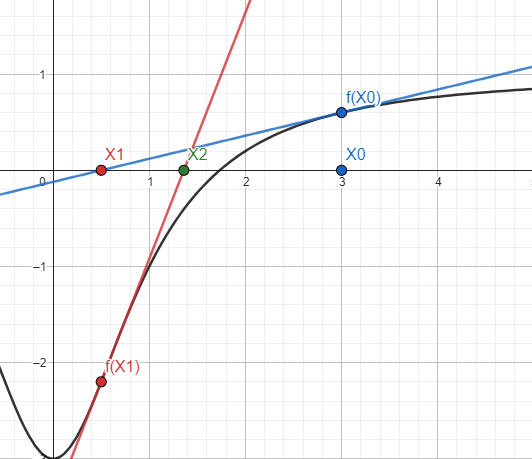
\includegraphics[scale=0.6]{img/tangent.png}
                \caption{Wizualizacja metody Newtona}
                \label{fig:tangent}
            \end{figure}

        \subsubsection*{Zadanie 3: Metoda siecznych}
            Metoda wyznacza kolejne przybliżenia pierwiastka funkcji $f$ jako argumenty punktów przecięcia z osią $x$ 
            siecznych funkcji $f$ w punktach $(x_n, f(x_n))$ oraz $(x_{n + 1}, f(x_{n + 1}))$ , zaczynając od zadanych
            przybliżeń początkowych $x_0$ i $x_1$. Kolejne przybliżenia są wyznaczane wg. wzoru
            $x_{n + 1} = x_n - f(x_n) \cdot \frac{x_n - x_{n - 1}}{f(x_n) - f(x_{n - 1})}$.
            Warunek końca metody siecznych jest taki sam, jak w metodzie Newtona - osiągnięcie wymaganej precyzji lub
            maksymalnej liczby iteracji.
            \newline
            \begin{figure}[h]
                \centering
                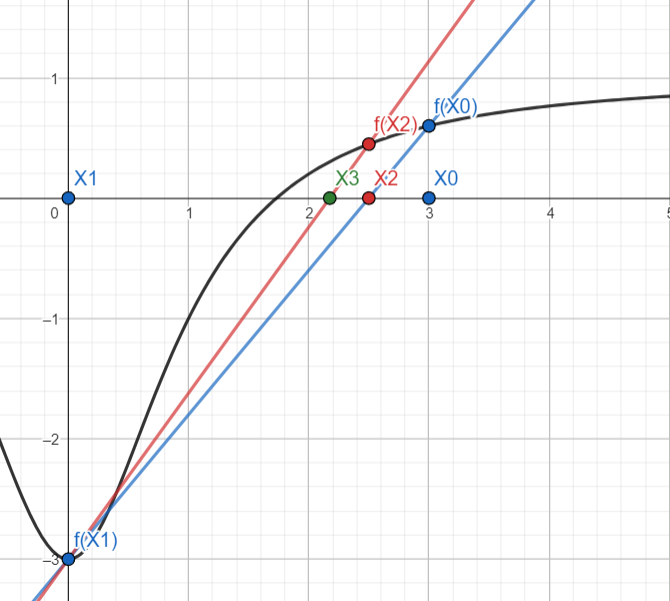
\includegraphics[scale=0.6]{img/secant.png}
                \caption{Wizualizacja metody siecznych}
                \label{fig:secant}
            \end{figure}

    \newpage
        
    \subsection*{Rozwiązanie}
        Program z rozwiązaniem: \texttt{solvers.jl}
        \newline
        Program z testami: \texttt{solvers\_test.jl}
        \newline\newline
        \textbf{Pseudokody badanych metod:}

        \begin{algorithm}
            \caption{Metoda bisekcji}\label{alg:bisection}
            \begin{algorithmic}[1]
                \Require $f, a, b, \delta, \varepsilon$
                \If{$sign(f(a)) = sign(f(b))$}
                    \Return $Error$
                \EndIf
                \State $d \gets b - a$
                \State $it \gets 0$
                \While{$true$}
                    \State $it \gets it + 1$
                    \State $d \gets \frac{d}{2}$
                    \State $c \gets a + d$
                    \If{$|d| < \delta$ or $|f(c)| < \varepsilon$}
                        \Return $(c, f(c), it, NoError)$
                    \EndIf
                    \If{$sign(f(a)) = sign(f(b))$}
                        \State $a \gets c$
                    \Else
                        \State $b \gets c$
                    \EndIf
                \EndWhile
            \end{algorithmic}
        \end{algorithm}

        \begin{algorithm}
            \caption{Metoda stycznych (Newtona)}\label{alg:tangend}
            \begin{algorithmic}[1]
                \Require $f, f', x_0, \delta, \varepsilon, M$ 
                    \Comment $M$ - maksymalna liczba iteracji
                \If{$|f(x_0)| < \varepsilon$}
                    \Return $Error$
                \EndIf
                \For{$it = 1$ to $M$}
                    \If{$|f'(x_0)| < \varepsilon$}
                        \Return $Error$
                    \EndIf
                    \State $x_1 \gets x_0 - \frac{f(x_0)}{f'(x_0)}$
                    \If{$|x_1 - x_0| < \delta$ or $|f(x_1)| < epsilon$}
                        \Return $(x_1, f(x_1), it, NoError)$
                    \EndIf
                    \State $x_0 \gets x_1$
                \EndFor
                \State \Return $Error$
            \end{algorithmic}
        \end{algorithm}

        \begin{algorithm}
            \caption{Metoda siecznych}\label{alg:secant}
            \begin{algorithmic}[1]
                \Require $f, x_0, x_1, \delta, \varepsilon, M$ \Comment $M$ - maksymalna liczba iteracji
                \For{$it = 1$ to $M$}
                    \If{$|f(x_0)| > |f(x_1)|$}
                        \State $(x_0, x_1) \gets (x_1, x_0)$
                    \EndIf
                    \State $s \gets \frac{x_1 - x_0}{f(x_1) - f(x_0)}$
                    \State $x_1 \gets x_0$
                    \State $x_0 \gets x_0 - f(a) \cdot s$
                    \If{$|x_1 - x_0| < \delta$ or $f(x_0) < \varepsilon$}
                        \Return $(x_0, f(x_0), it, NoError)$
                    \EndIf
                \EndFor
                \State \Return $Error$
            \end{algorithmic}
        \end{algorithm}

    \newpage

\section*{Zadanie 4: Wyznaczanie pierwiastków}
    \subsection*{Problem}
        Za pomocą zaimplementowanych metod z zadań 1-3 wyznaczyć znaleźć przybliżenie pierwiastka
        funkcji $f(x) = \sin{x} - (\frac{x}{2})^2$ dla dokładności obliczeń 
        $\delta = \varepsilon = \frac{1}{2} \cdot 10^{-5}$ oraz dla zadanych danych:
        \begin{itemize}
            \item Metoda bisekcji: $a = 1.5 \land b = 2$
            \item Metoda stycznych: $x_0 = 1.5$
            \item Metoda siecznych: $x_0 = 1 \land x_1 = 2$
        \end{itemize}

    \subsection*{Rozwiązanie}
        Policzmy pochodną funkcji $f$ wymaganą dla metody Newtona:
        \begin{center}
        \begin{math}
            f'(x) = \frac{d}{dx}(\sin{x} - (\frac{x}{2})^2) 
                = \frac{d}{dx}\sin{x} - \frac{d}{dx}(\frac{x}{2})^2
                = \cos{x} - \frac{x}{2}
        \end{math}
        \end{center}
        \noindent \newline
        Program z rozwiązaniem: \texttt{ex4.jl}
        
    \subsection*{Wyniki i obserwacje}
        Na podstawie \textit{tabeli 1} możemy zauważyć, że wszystkie badane metody zwracają poprawne przybliżenia 
        pierwiastka funkcji $f$ z założoną dokładnością. Można też zauważyć, że metoda Newtona zwróciła wynik w 
        najmniejszej liczbie iteracji $it_n = 4$, natomiast metoda bisekcji potrzebowała $it_b = it_n^2$ iteracji.
        Metoda stycznych potrzebowała $it_n < it_s = 5 < it_b$ iteracji. Jest to oczekiwany wynik, biorąc pod uwagę
        wartości współczynników zbieżności $\alpha$ dla badanych metod: $\alpha_n = 2$ (zbieżność kwadratowa), 
        $\alpha_s = \frac{1 + \sqrt{5}}{2} \approx 1.1618$ oraz $\alpha_b = 1$ (zbieżność liniowa).

        \begin{table}[h!]
        \centering
        \begin{tabularx}{0.7\textwidth}{l l l l l }
            \hline
            Metoda & $r$ & $v$ & $it$ & $err$ \\
            \hline
            Bisekcji & $1.9337539672851562$ & $-2.7027680138402843e-7$ & $16$ & $0$ \\
            Stycznych & $1.933753779789742$ & $-2.2423316314856834e-8$ & $4$ & $0$ \\
            Siecznych & $1.9337537628211916$ & $7.706280058528137e-12$ & $5$ & $0$ \\
            \hline
        \end{tabularx}
        \label{table:ex4}
        \caption{Wyniki badanych metod iteracyjnych dla funkcji $f(x) = \sin{x} - (\frac{x}{2})^2$}
        \end{table}

\section*{Zadanie 5: Przecięcie funkcji}
    \subsection*{Problem}
        Za pomocą metody biseckji znaleźć argument $x$ dla którego funkcje $f_1(x) = 3x$ oraz 
        $f_2(x) = e^x$ się przecinają, zakładając dokładność obliczeń $\delta = \varepsilon = 10^{-4}$

    \subsection*{Rozwiązanie}
        Punkt przecięcia funkcji $f_1$ oraz $f_2$ możemy wyznaczyć obliczając pierwiastek funkcji
        $f(x) = f_1(x) - f_2(x)$.
        \newline
        Wynikiem będzie zatem przybliżenie rozwiązań równania $3x - e^x = 0$. 
        Wiemy, że prawdziwe pierwiastki tego równania leżą w przedziałach $[0, 1]$ ($f(0) = -1 \land f(1) = 3 - e \approx 0.28$) 
        oraz $[1, 2]$ ($f(1) = 3 - e \land f(2) = 6 - e^2 \approx -1.39$),
        zatem dla takich przedziałów będziemy wywoływać metodę bisekcji.
        \newline\newline
        Program z rozwiązaniem: \texttt{ex5.jl}
        
    \subsection*{Wyniki i obserwacje}
        \begin{table}[h!]
        \centering
        \begin{tabularx}{0.7\textwidth}{l l l l l }
            \hline
            Przedział & $r$ & $v$ & $it$ & $err$ \\
            \hline
            $[0, 1]$ & $x_1 = 0.619140625$ & $9.066320343276146e-5$ & $9$ & $0$ \\
            $[1, 2]$ & $x_2 = 1.5120849609375$ & $9.066320343276146e-5$ & $13$ & $0$ \\
            \hline
        \end{tabularx}
        \label{table:ex5}
        \caption{Wyniki metody bisekcji dla problemu wyznaczenia punktu przecięcia dwóch funkcji}
        \end{table}

        \noindent Widzimy, że metoda nie zwraca sygnału o błędzie oraz otrzymane wyniki spełniają rządane warunki co do
        dokładności przybliżeń. Możemy zatem określić przybliżenia punktów przecięcia funkcji $f_1$ i $f_2$, jako
        $(x_1, f^*(x_1))$ oraz $(x_2, f^*(x_2))$, gdzie $f^*$ jest dowolną z funkcji $f_1$, $f_2$.Metoda ta wymaga jednak
        wcześniejszej analizy przebiegu funkcji, by móc poprawnie określić parametry startowe $a$ oraz $b$.

        \noindent\newline

\section*{Zadanie 6: Wyznaczanie pierwiastków}
    \subsection*{Problem}
        Za pomocą zaimplementowanych metod z zadań 1-3 wyznaczyć znaleźć przybliżenie pierwiastków
        funkcji $f_1(x) = e^{1 - x} - 1$ oraz $f_2(x) = x \cdot e^{-x}$ dla dokładności obliczeń 
        $\delta = \varepsilon = \cdot 10^{-5}$.
        \newline
        Dla każdej metody należy dobrać odpowiednie dane wejściowe oraz sprawdzić, jaki będzie wynik metody
        Newtona dla funkcji $f_1$ oraz $x_0 \in (1, \infty]$, a także dla $x_0 > 1$ i $x_0 = 1$ dla funkcji $f_2$.
        \newline

    \subsection*{Rozwiązanie}
        Policzmy pochodne funkcji $f_1$ oraz $f_2$ wymagane dla metody Newtona:
        \begin{center}
        \begin{math}
            f_1'(x) = \frac{d}{dx}(e^{1 - x} - 1) = -e^{1 - x}
        \end{math}
        \end{center}
        \noindent
        \begin{center}
        \begin{math}
            f_2'(x) = \frac{d}{dx}(x \cdot e^{-x}) = x \cdot (-e^{-x}) + e^{-x} = e^{-x} \cdot (1 - x)
        \end{math}
        \end{center}
        \noindent\newline
        Program z rozwiązaniem: \texttt{ex6.jl}
        
    \subsection*{Wyniki i obserwacje}
        W \textit{tabelach 3} i  \textit{4} widzimy, że dla odpowiednio dobranych parametrów startowych wszystkie badane
        metody zwracają poprawne przybliżenia (z założoną dokładnością) dla obu funkcji $f_1$ i $f_2$. Dodatkowo zauważmy,
        że najbardziej dokładne przybliżenia zwraca metoda siecznych.
        \newline\newline
        Badając wyniki metody Newtona dla funkcji $f_1$, możemy zaobserwować, że wybranie wartości 
        $x_0 \in (1, \infty]$ powoduje bardzo szybki wzrost liczby iteracji potrzebnej do osiągnięcia
        założonej precyzji - dla $x_0 = 6$ potrzebujemy aż $147$ iteracji. Wynika to z faktu, że funkcja $g_1(x) = e^{1 - x}$ 
        ($f_1(x) = g_1(x) - 1$) bardzo szybko zbiega do $0$, zatem styczne do niej w punktach $x_0 \in (1, \infty]$ są 
        "bliskie funkcji stałej" (pochodne są bliskie $0$), więc kolejne wartości $x_n$ są bardzo nieznacznie od siebie oddalone.
        \newline
        Dla funkcji $f_2$ możemy zauważyć, że przyjęcie przybliżenia początkowego $x_0 \geq 1$ skutkuje otrzymaniem 
        niepoprawnych wyników ($\geq \sim 14.4$), gdzie jedynym pierwiastkiem tej funkcji jest $0$. Jest to skutkiem
        zmiany monotoniczności funkcji w punkcie $x_0 = 1$ - funckja w nieskończoności zbiega do $0$. Wyznaczając zatem
        kolejne przybliżenia pierwiastka funkcji coraz bardziej oddalamy sie od rzeczywistej wartości podobnie jak dla funkcji
        $f_1$, w pewnym momencie osiągając wartość $f_2(x_n) \approx 0$, co kończy działanie metody z błędnym wynikiem.

        \begin{table}[h!]
        \centering
        \begin{tabularx}{0.88\textwidth}{l l l l l l }
            \hline
            Metoda & Parametry & $r$ & $v$ & $it$ & $err$ \\
            \hline
            Bisekcji & $a = 0 \land b = 3$ & $1.0000076293945312$ & $-7.6293654275305656e-6$ & $17$ & $0$ \\
            Stycznych & $x_0 = e^{-1}$ & $0.9999999967966953$ & $3.2033047325796815e-9$ & $4$ & $0$ \\
            Siecznych & $x_1 = 0 \land x_2 = 3$ & $1.0000000003101366$ & $-3.101365830815439e-10$ & $7$ & $0$ \\
            \hline
        \end{tabularx}
        \label{table:ex6_f1}
        \caption{Wyniki badanych metod iteracyjnych dla funkcji $f_1(x) = e^{1 - x} - 1$}
        \end{table}

        \begin{table}[h!]
        \centering
        \begin{tabularx}{0.965\textwidth}{l l l l l l }
            \hline
            Metoda & Parametry & $r$ & $v$ & $it$ & $err$ \\
            \hline
            Bisekcji & $a = -1 \land b = 2$ & $7.629394531248679e-6$ & $7.629336323809809e-6$ & $16$ & $0$ \\
            Stycznych & $x_0 = e^{-1}$ & $-1.8840380756452411e-6$ & $-1.8840416252480553e-6$ & $4$ & $0$ \\
            Siecznych & $x_1 = -1 \land x_2 = 1$ & $2.7077871812544315e-13$ & $2.7077871812536984e-13$ & $19$ & $0$ \\
            \hline
        \end{tabularx}
        \label{table:ex6_f2}
        \caption{Wyniki badanych metod iteracyjnych dla funkcji $f_2(x) = x \cdot e^{-x}$}
        \end{table}

        \newpage

        \begin{table}[h!]
        \centering
        \begin{tabularx}{0.63\textwidth}{l l l l l }
            \hline
            $x0$ & $r$ & $v$ & $it$ & $err$ \\
            \hline
            $2$ & $0.9999999810061002$ & $1.8993900008368314e-8$ & $5$ & $0$ \\
            $3$ & $0.9999999710783241$ & $2.892167638712806e-8$ & $9$ & $0$ \\
            $4$ & $0.9999999995278234$ & $4.721767421500545e-10$ & $21$ & $0$ \\
            $5$ & $0.9999996427095682$ & $3.572904956339329e-7$ & $54$ & $0$ \\
            $6$ & $0.9999999573590406$ & $4.264096031825204e-8$ & $147$ & $0$ \\
            $7$ & $0.0$ & $0.0$ & $256$ & $1$ \\
            $8$ & $0.0$ & $0.0$ & $256$ & $1$ \\
            $9$ & $0.0$ & $0.0$ & $256$ & $1$ \\
            $10$ & $0.0$ & $0.0$ & $256$ & $1$ \\
            \hline
        \end{tabularx}
        \label{table:ex6_newton_f1}
        \caption{Wyniki metody Newtona dla funkcji $f_1(x) = e^{1 - x} - 1$ oraz wybranych wartości $x_0 \in (1, \infty]$}
        \end{table}

        \begin{table}[h!]
        \centering
        \begin{tabularx}{0.625\textwidth}{l l l l l }
            \hline
            $x0$ & $r$ & $v$ & $it$ & $err$ \\
            \hline
            $2$ & $14.398662765680003$ & $8.03641534421721e-6$ & $10$ & $0$ \\
            $3$ & $14.787436802837927$ & $5.594878975694858e-6$ & $10$ & $0$ \\
            $4$ & $14.398662765680003$ & $8.03641534421721e-6$ & $9$ & $0$ \\
            $5$ & $15.194283983439147$ & $3.827247505782993e-6$ & $9$ & $0$ \\
            $6$ & $14.97432014974184$ & $4.699833827208111e-6$ & $8$ & $0$ \\
            $7$ & $14.792276940955892$ & $5.569686859646652e-6$ & $7$ & $0$ \\
            $8$ & $14.636807965014$ & $6.438155219843286e-6$ & $6$ & $0$ \\
            $9$ & $14.50105208065629$ & $7.305881300498495e-6$ & $5$ & $0$ \\
            $10$ & $14.380524159896261$ & $8.173205649825554e-6$ & $4$ & $0$ \\
            $11$ & $14.272123938290518$ & $9.040322779745372e-6$ & $3$ & $0$ \\
            $12$ & $14.173615857826384$ & $9.907349924182477e-6$ & $2$ & $0$ \\
            $13$ & $15.159766454352443$ & $3.95266121872815e-6$ & $2$ & $0$ \\
            $14$ & $15.076923076923077$ & $4.270593381508261e-6$ & $1$ & $0$ \\
            $15$ & $15.0$ & $4.588534807527386e-6$ & $0$ & $0$ \\
            $16$ & $16.0$ & $1.8005627955081459e-6$ & $0$ & $0$ \\
            $17$ & $17.0$ & $7.037894121934784e-7$ & $0$ & $0$ \\
            $18$ & $18.0$ & $2.741396354048273e-7$ & $0$ & $0$ \\
            $19$ & $19.0$ & $1.0645313231320808e-7$ & $0$ & $0$ \\
            $20$ & $20.0$ & $4.122307244877116e-8$ & $0$ & $0$ \\
            \hline
        \end{tabularx}
        \label{table:ex6_newton_f2}
        \caption{Wyniki metody Newtona dla funkcji $f_1(x) = e^{1 - x} - 1$ oraz wybranych wartości $x_0 \geq 1$}
        \end{table}     
        
        \newpage

        \begin{figure}
            \centering
            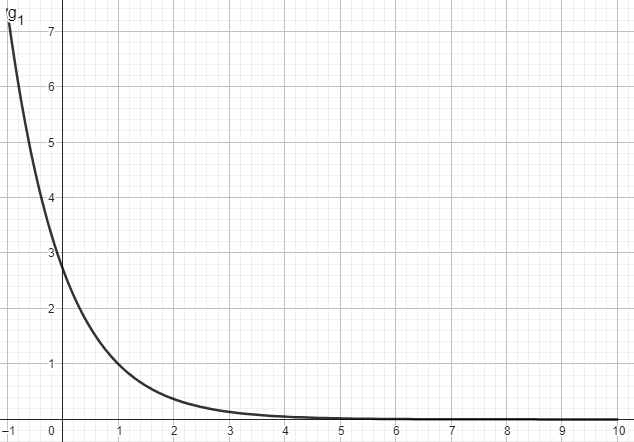
\includegraphics[width=0.8\textwidth]{img/ex6_g1.png}
            \caption{Funkcja $g_1(x) = e^{1 - x}$}
            \label{fig:ex6_g1}
        \end{figure}

        \begin{figure}
            \centering
            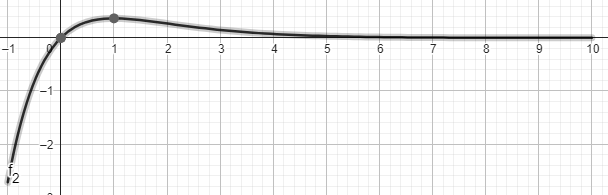
\includegraphics[width=0.8\textwidth]{img/ex6_f2.png}
            \caption{Funkcja $f_2(x) = x \cdot e^{x}$}
            \label{fig:ex6_f2}
        \end{figure}

\end{document}
